\documentclass[11pt, oneside]{article} 
\usepackage{geometry}
\geometry{letterpaper} 
\usepackage{graphicx}
	
\usepackage{amssymb}
\usepackage{amsmath}
\usepackage{parskip}
\usepackage{color}
\usepackage{hyperref}

\graphicspath{{/Users/telliott_admin/Dropbox/Tex/png/}}
% \begin{center} 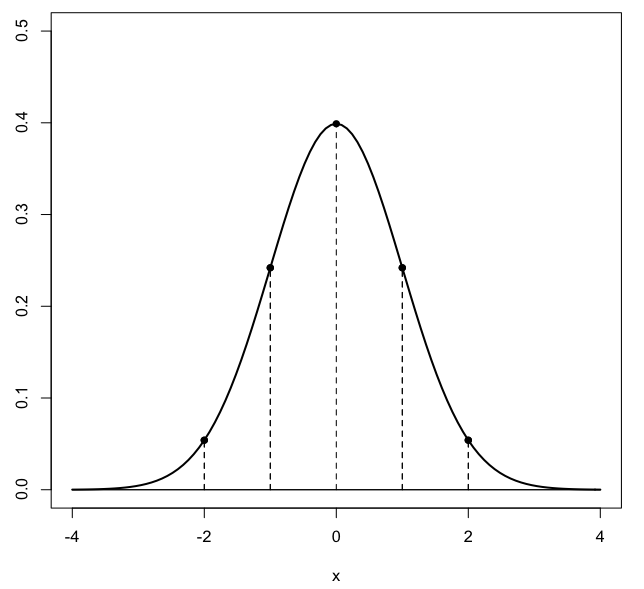
\includegraphics [scale=0.4] {gauss3.png} \end{center}

\title{Orthocenter}
\date{}

\begin{document}
\maketitle
\Large
In this write-up we look at the properties of the orthocenter, which is the point where the three altitudes of a triangle meet.  For an acute triangle, the orthocenter is inside the triangle.  We assume for now that the three altitudes \emph{do} meet at a single point, we will come back to this later.
\begin{center} 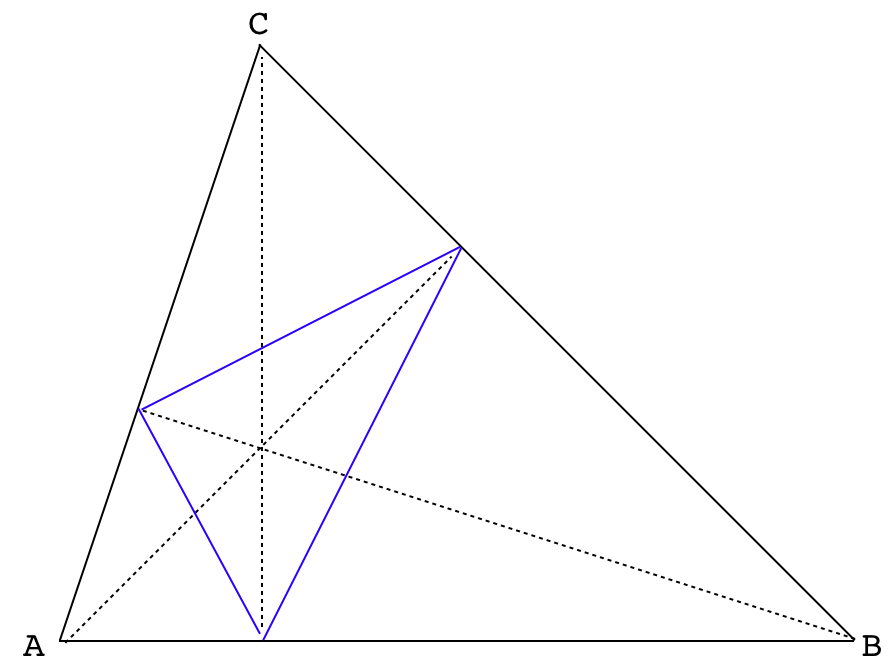
\includegraphics [scale=0.25] {ortho1.png} \end{center}
Here the altitudes are drawn as dotted lines, and we have also connected the points where these lines meet their opposite sides, to form another triangle outlined in blue.

Recall that the same construction for the centroid yielded four small triangles which are all congruent.  In the case of the orthocenter, we will show that the three outer triangles are similar (though obviously not congruent), while the one in the center is different.

The first observation is that the angles $A$, $B$, and $C$ are divided by the altitudes into two parts with the measures repeated as shown.  Proof:  there are two right triangles formed that include $A$ as a base angle.  The corresponding complementary angles must be equal, and these are labeled $\gamma$.  A similar argument gives $\alpha$ and $\beta$.
\begin{center} 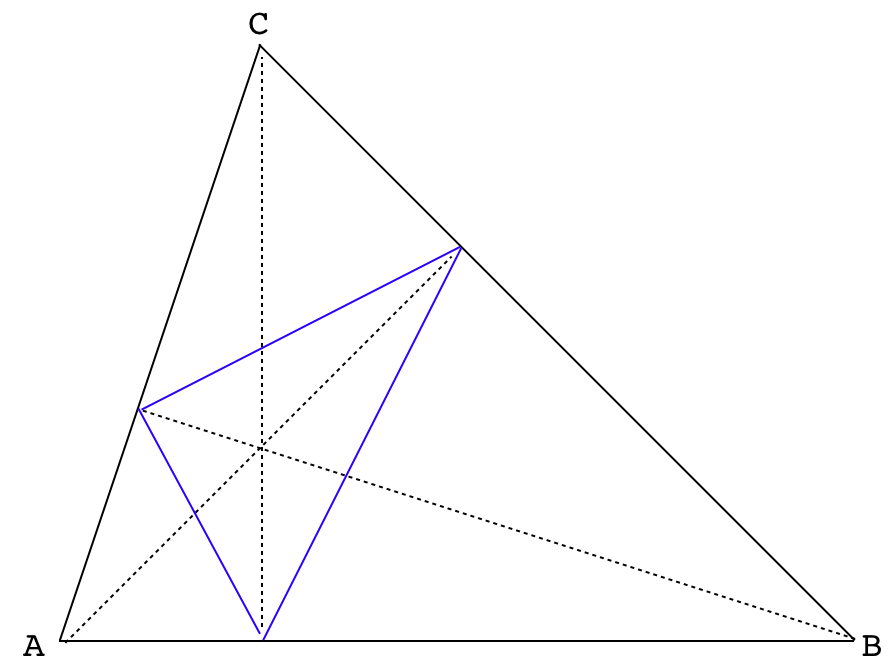
\includegraphics [scale=0.3] {ortho1.png} \end{center}
Switching our attention to the central angles, we can show that these have measures equal to the vertices, as shown in the next diagram.
\begin{center} 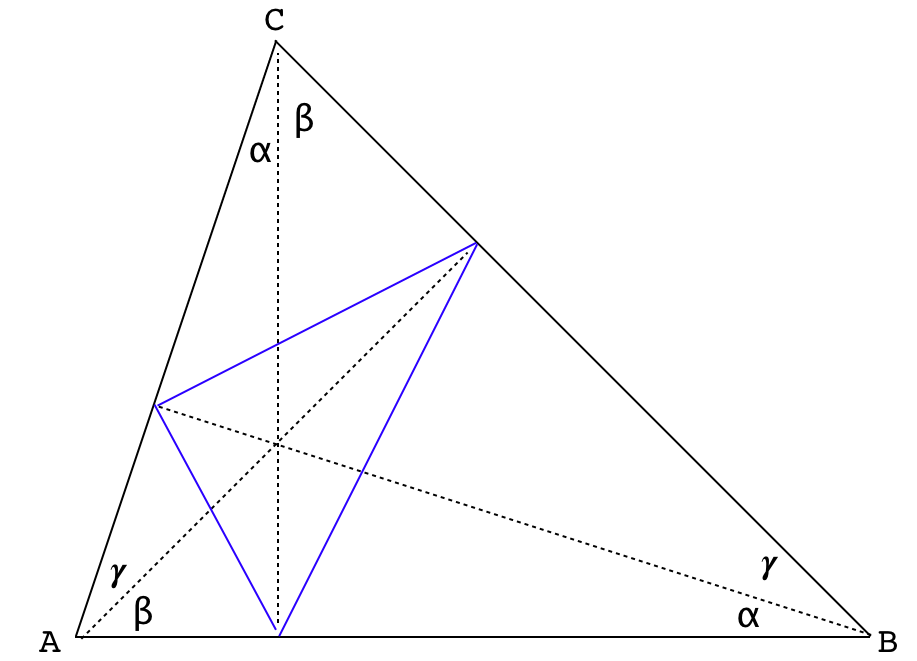
\includegraphics [scale=0.3] {ortho2.png} \end{center}
The argument builds on the one above, each central angle is part of a right triangle with one of $\alpha$, $\beta$, or $\gamma$ as the complementary angle.

At this point, it is my duty to acknowledge that there is an easy way and a hard way of doing what follows.  We start with the hard way.

The next fact that we need is that the altitudes are angle bisectors for the inscribed triangle.   This is a bit of a challenge, we will prove it near the end.

It will turn out later that the half-angles are the quantities ($\alpha$, $\beta$ and $\gamma$) that we already know, but for now we label them $x$, $y$ and $z$.  Note that $2x + 2y + 2z = 180$, so $x + y + z = 90$.
\begin{center} 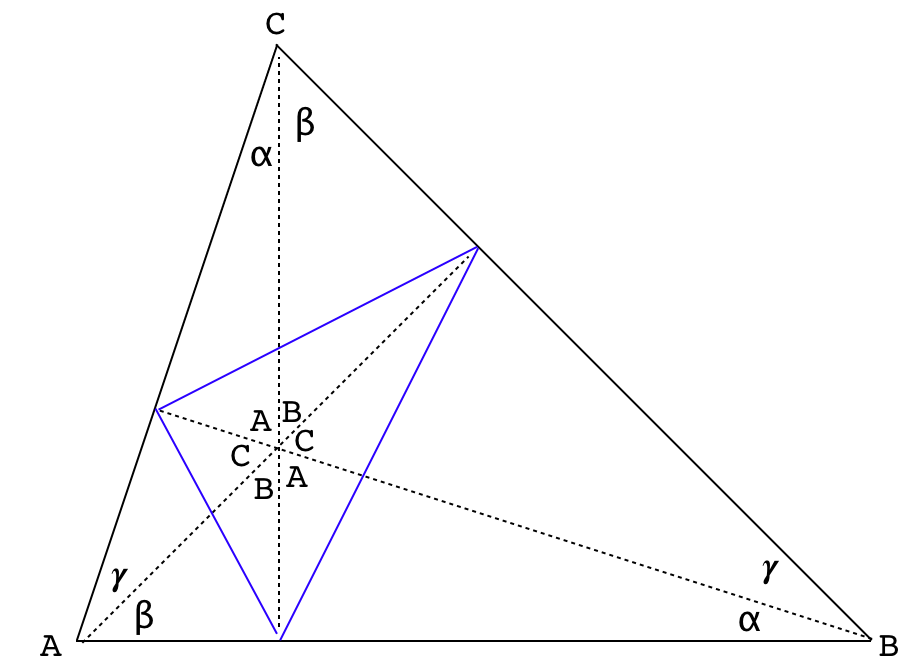
\includegraphics [scale=0.3] {ortho3.png} \end{center}

At this point, we use the properties of vertical and supplementary angles to label a few more of the angles in the diagram.  Consider the quadrilateral formed around the part of the altitude from the orthocenter extending up to the side BC.  Let's count up the angles included in this quadrilateral:
\[ C + B + A + z + x + x + A + y = 360 \]
\[ z + x + x + A + y = 180 \]
Since $ x + y + z = 90$
\[ A + x = 90 \]
This shows that $x = \gamma$.

In a similar way, for the quadrilateral extending down from the orthocenter to the base we add up
\[ A + C + x + y + y + C + z + B = 360 \]
\[ x + y + y + C + z = 180 \]
\[ y + C = 90 \]
\[ y = \beta \] 
Since $x + y + z = \alpha + \beta + \gamma$, we conclude that the third angle is $z = \alpha$.
\begin{center} 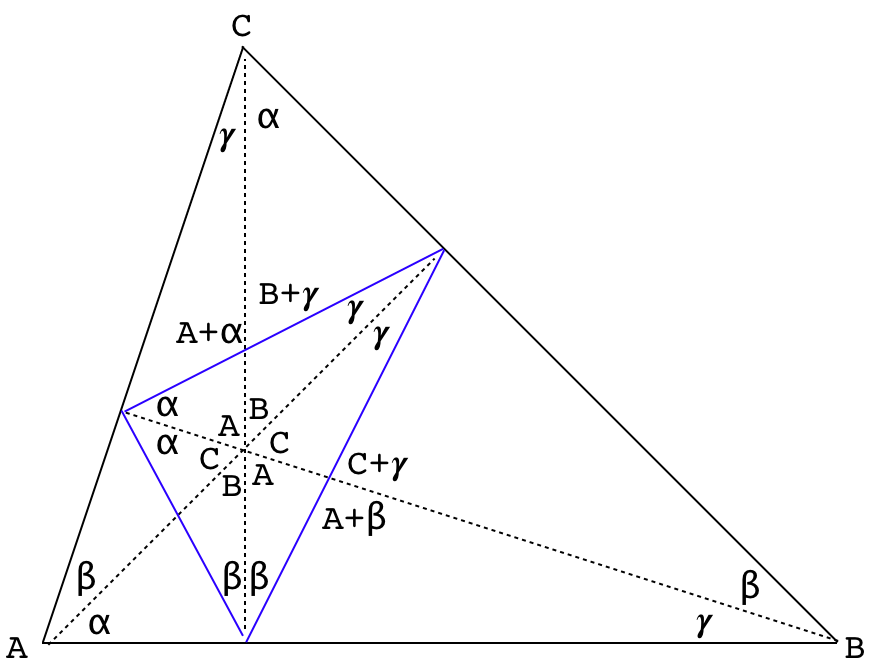
\includegraphics [scale=0.3] {ortho4.png} \end{center}
Finally we use complementary angles again:
\begin{center} 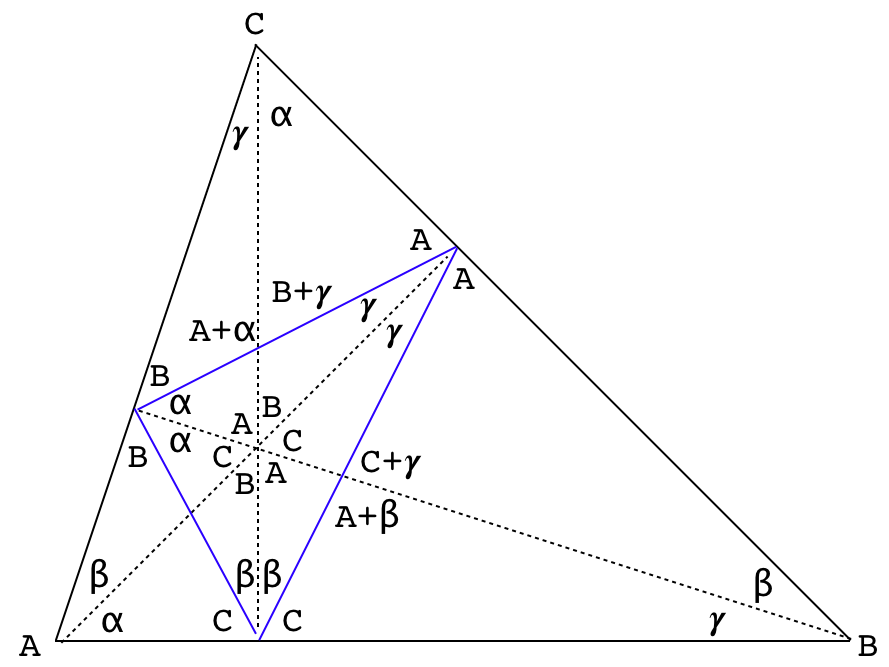
\includegraphics [scale=0.3] {ortho5.png} \end{center}
Clean it up a bit:
\begin{center} 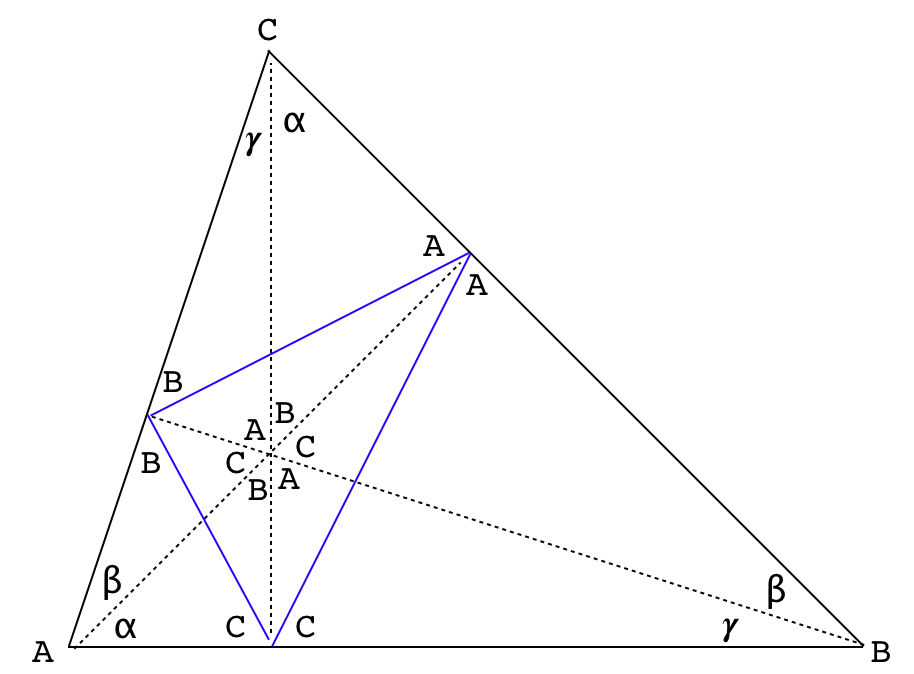
\includegraphics [scale=0.3] {ortho7.png} \end{center}
It's clear that the three small triangles which each include one vertex are similar.

\subsection*{Orthocenter exists}
For the above derivation, we assumed that the three altitudes do indeed meet at a single point.  This is a direct consequence of Ceva's Theorem, which we've seen before.  Below is an alternative proof, due to Euler, which is stunning.  We will also need to show that the altitudes are bisectors of the angles in the central triangle.

For the first one, we follow

\url{https://artofproblemsolving.com/wiki/index.php/Orthocenter}

Borrowing their figure:
\begin{center} 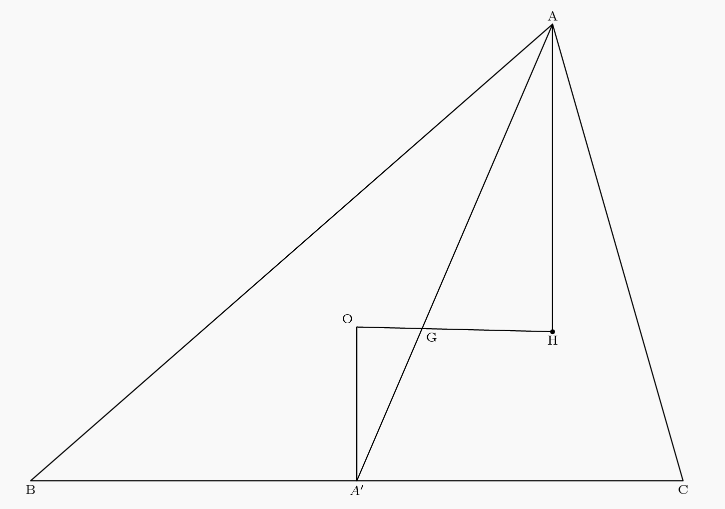
\includegraphics [scale=0.4] {circumcenter.png} \end{center}
The orientation is reversed from what we had above.  First, the point $O$ is the circumcenter of the triangle:  the center of the circle which contains all three vertices of the triangle.  Clearly this circle  has a center.

The classic construction is to bisect each side (here $BC$ is bisected at $A'$), and erect a perpendicular.  The point where the three perpendiculars cross is the circumcenter, which is the center of the circle.  So, assume we have done this and that point is $O$.

The next point, $G$, is the centroid.  One way to find this point is to draw all three lines connecting vertices with the midpoints of the opposite side ($AA'$).  However, if you recall, the distance from the vertex $A$ to $G$ is twice the distance from the midpoint $A'$ to $G$.  Hence we draw point $G$ using arithmetic.

Now, extend $OG$ by twice its length, to $H$.  ($2OG = GH$).
\begin{center} 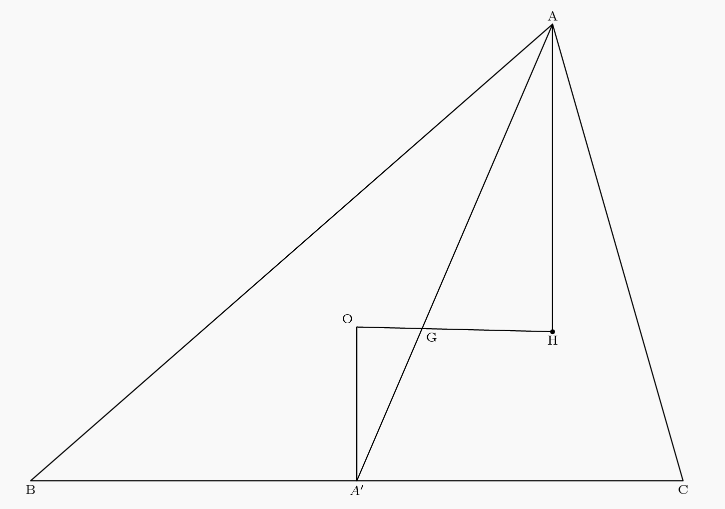
\includegraphics [scale=0.4] {circumcenter.png} \end{center}
Because $AG$ is twice $A'G$ and $GH$ is twice $OG$ and the two triangles share both angle $\angle OGA'$ (equal to $\angle AGH$), they are similar triangles.  

Since $\angle A'OG$ is a right angle, therefore so is $\angle AHG$.  This means that $AH$ is perpendicular to $BC$.  Thus, $AH$ is a part of the altitude from $A$ to $BC$ (the whole altitude is not shown).

The same construction could be done for the other two vertices, each time ending at $H$.  This shows that $H$ is unique, and that $H$ is on all three altitudes.

This proof also demonstrates that the orthocenter, centroid and circumcenter lie on a single line, and that the distance from centroid to orthocenter is twice that from centroid to circumcenter.

\subsection*{Angle bisection}
Here we follow

\url{https://sites.math.washington.edu/~king/coursedir/m444a04/notes/orthic/www/Altitudes%20and%20Orthic%20Tri.htm}
\begin{center} 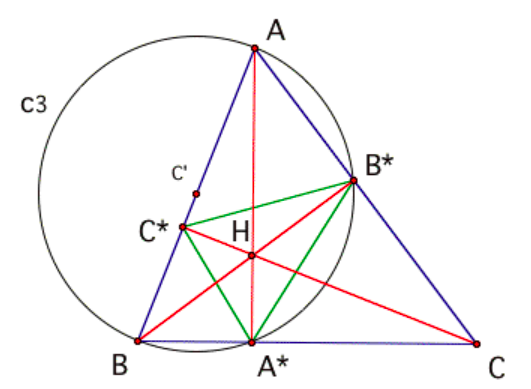
\includegraphics [scale=0.45] {bisector1.png} \end{center}
The angles on this figure are also labeled differently than ours, but we will be able to look at similar parts.

First, draw the circle that has $AB$ as its diameter.  We will show that this circle also passes through $B*$ and $A*$, where the altitudes meet their respective opposing sides.

We know that (for example) $\angle AB^*B$ is a right angle because $BB*$ is an altitude of the triangle $\triangle ABC$.  On the other hand, $\angle AB^*B$ forms a right angle if and only if $B*$ lies on the circle.  Therefore $B*$ lies on the circle.  Now consider
\begin{center} 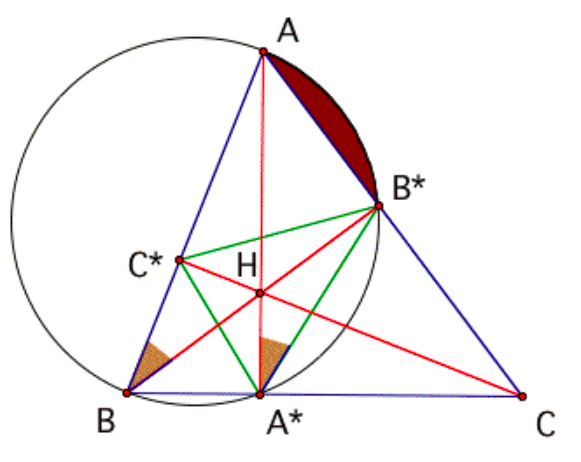
\includegraphics [scale=0.4] {bisector2.png} \end{center}

By a famous theorem, because these two angles (shaded light brown) have their vertices on the circle and they subtend the same arc of the circle, they are themselves equal.  If we look again at our original figure at this stage in the argument, one of those angles is known to have measure $\beta$, therefore we label the other the same  (in red):
\begin{center} 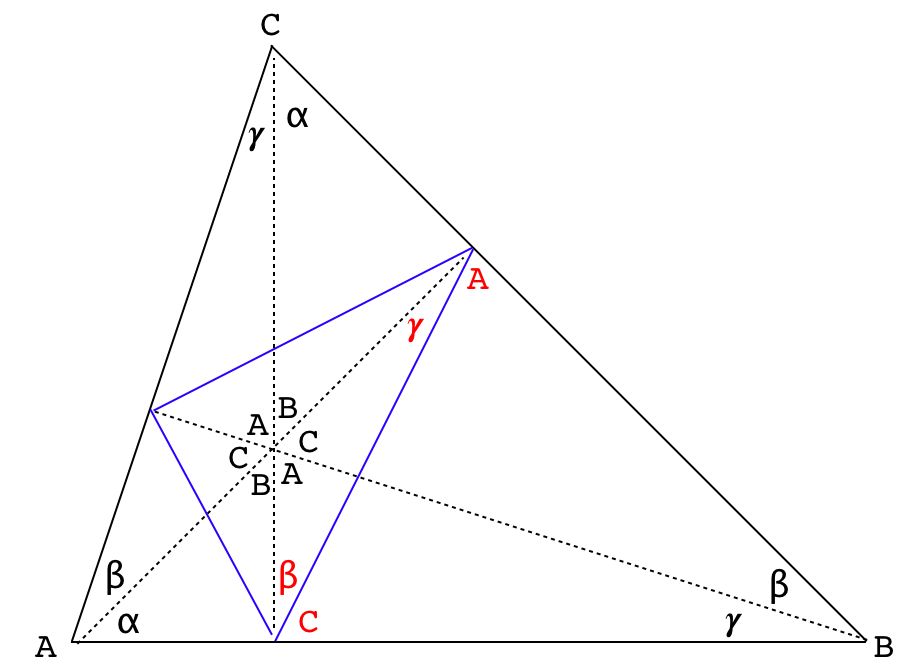
\includegraphics [scale=0.3] {ortho8.png} \end{center}
As a consequence, we immediately obtain the other angles shown in red.

We could draw another circle, but there is nothing special about the two vertices we chose to make the circle.  Therefore, by symmetry, it is clear that the angle $\alpha$ must be as shown on the inner triangle in the next figure.
\begin{center} 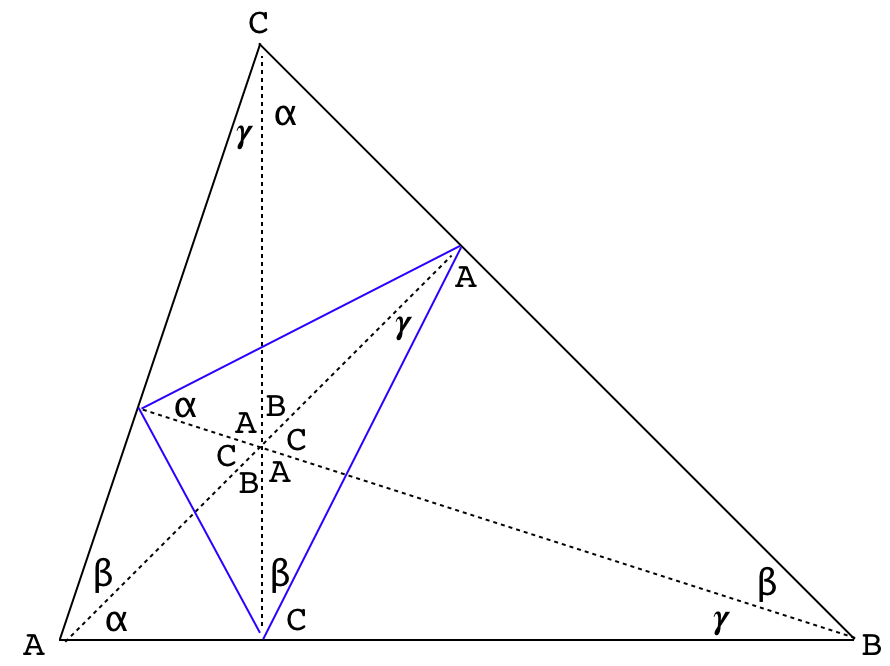
\includegraphics [scale=0.3] {ortho9.png} \end{center}

Finally, looking one last time at
\begin{center} 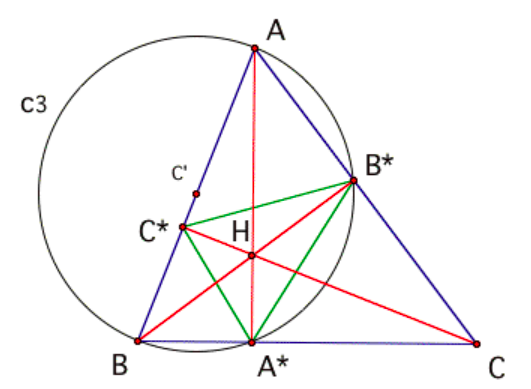
\includegraphics [scale=0.45] {bisector1.png} \end{center}
we notice that $\angle A^*C^*B^*$ subtends the same arc as $\angle A^*AB^*$ but is at the center of the circle, therefore the measure of the angle is twice the latter, or twice $\alpha$.  Since one part of the angle corresponding to $\angle A^*C^*B^*$ is already labeled $\alpha$ in our diagram, we must have that the second part is equal to $\alpha$ as well.
\begin{center} 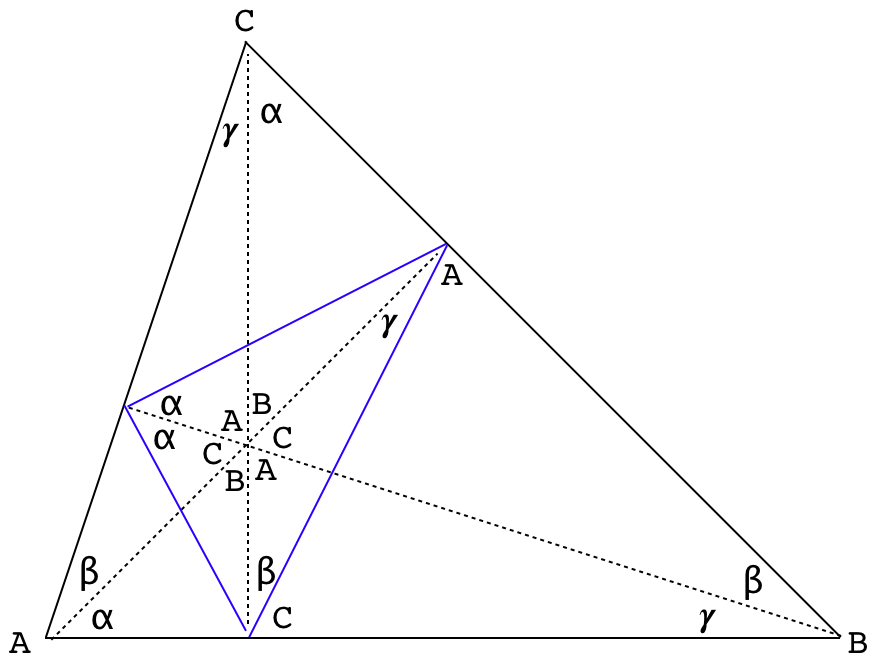
\includegraphics [scale=0.3] {ortho10.png} \end{center}
From this point, we can fill in everything using angle arithmetic.

\subsection*{Short and sweet}
Here is a much quicker proof from Courant and Robbins.
\begin{center} 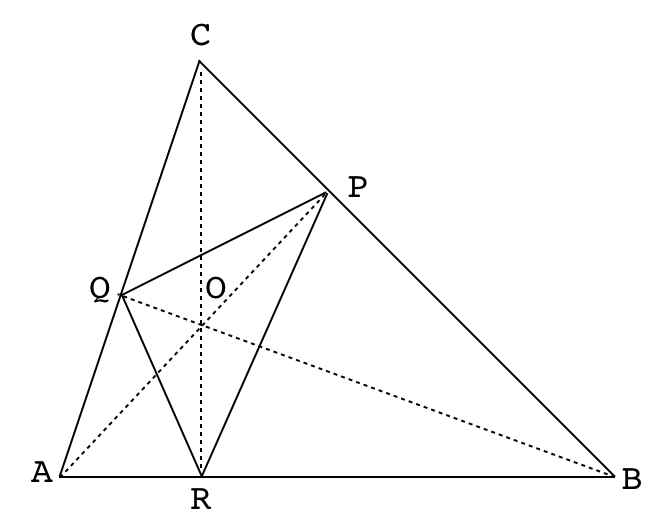
\includegraphics [scale=0.4] {ortho11.png} \end{center}
Since $\angle OPB$ is a right angle and so is $\angle ORB$, the quadrilateral $OPBR$ containing both can be inscribed into a circle with $OB$ as the diameter.

\begin{center} 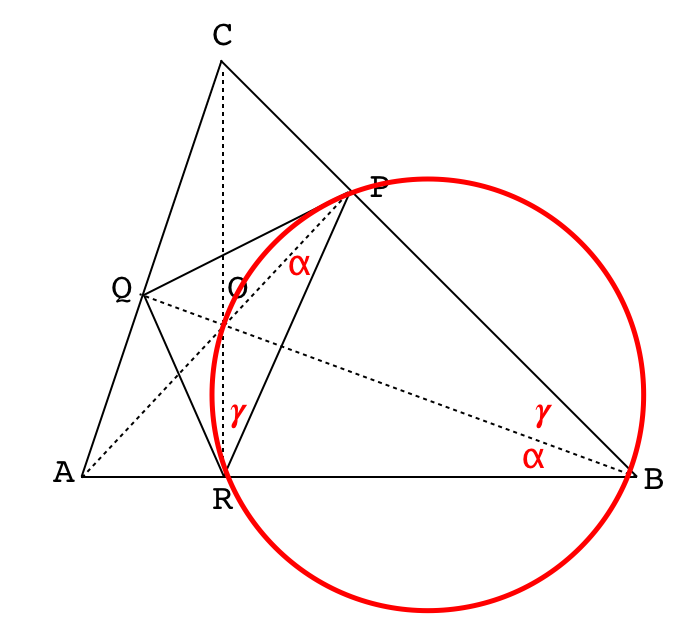
\includegraphics [scale=0.35] {ortho12.png} \end{center}
This immediately allows labeling of $\beta$ and $\gamma$ as shown in the diagram, and by comparison with triangle $\triangle ABQ$ we find that $A$ is the complement of $\gamma$.
\begin{center} 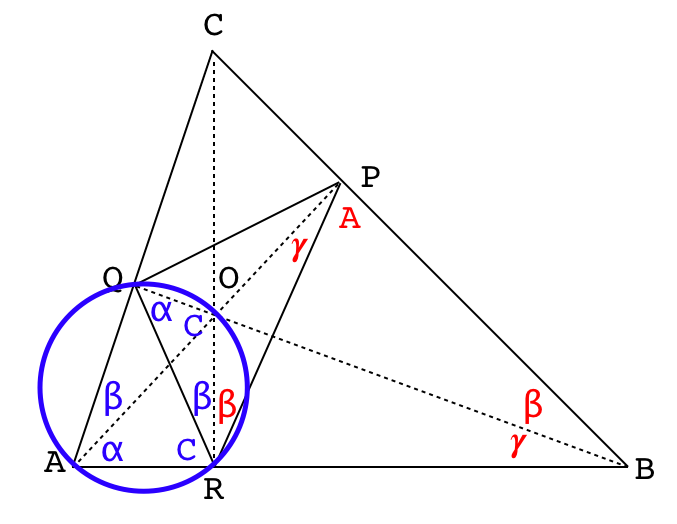
\includegraphics [scale=0.4] {ortho13.png} \end{center}
We also see that given the identities of the central angles, we can find that the vertex angle $C$, for example, is equal to $\angle ARQ$.  But such analysis is really unnecessary, once we know that $\angle CRQ = \beta$.

\subsection*{a famous theorem}
We have used this theorem twice: if two angles have their vertices on the circle and they subtend equal arcs of the circle, they are themselves equal.  I actually don't know what it's called, but I thought it important to come up with a proof.
\begin{center} 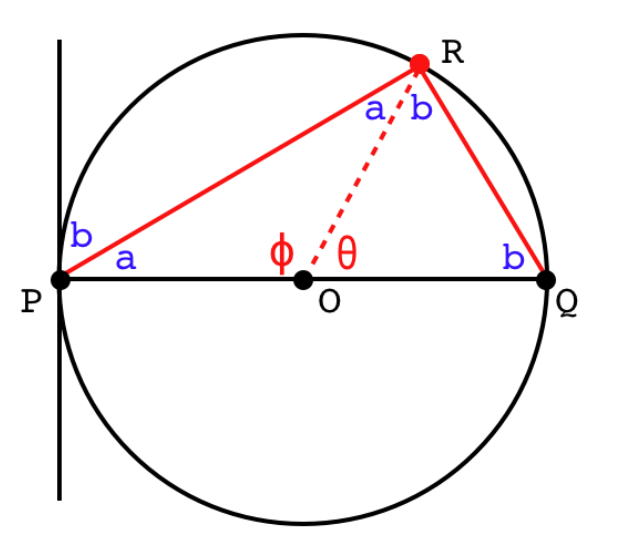
\includegraphics [scale=0.3] {diameter_angles.png} \end{center}

First of all, this sketch is for a proof that should be familiar:  if we take any diameter and a third point on the circle, then the vertex at that point $R$ is a right angle.  The proof is simple:  $OQ$ and $OR$ are equal in length (because they are radii of the circle) so $\triangle OQR$ is isosceles with equal base angles we can label $b$.  By the same argument we can label the two angles $a$.  But now $2a + 2b = 180$ so $a + b = 90$.

\begin{center} 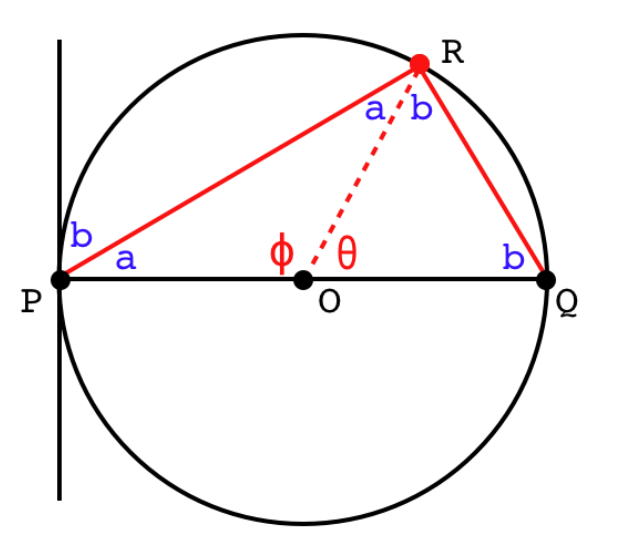
\includegraphics [scale=0.3] {diameter_angles.png} \end{center}

Furthermore, $2b + \theta = 180$, so $\theta = 2a$ and $a = \frac{1}{2} \theta$.

Now, consider angle $a$ and the arc it subtends $RQ$.  This is the same length subtended by angle $\theta$, and the arc is by definition equal to $\theta$ which is equal to $2a$.  Hence the arc subtended by any angle $a$ on the circle is equal to $2a$, provided that one of the lines meeting at $a$ is a diameter of the circle.

To make the argument completely general, if angle $a$ includes the center of the circle, divide $a$ into two angles with a diameter and apply the theorem separately to each part, then add.  

Alternatively, if $a$ is too small, construct another angle $c$ adjacent to it such that $a + c$ has one side on the diameter.  

In either case, we find that the angle at a point on the circumference, corresponding to a given subtended arc is one-half the arc.  Therefore, two angles that subtend the same arc are equal in measure.
 
\end{document}